% PQC-LINK progress report, Phase 1 (computer-only link).
%
% Build (any LaTeX with TikZ and pgfplots):   latexmk -pdf progress_report.tex
% Regenerate the plot data from the raw benchmark CSVs first:
%   python3 -I prepare_data.py ../../results data
% Every number in the results section comes from data/numbers.tex, which that script writes
% from the raw files. Do not type measurements into this file.
\documentclass[11pt,a4paper]{article}

\usepackage[margin=2.2cm]{geometry}
\usepackage[T1]{fontenc}
\usepackage{lmodern}
\usepackage{microtype}
\usepackage{xcolor}
\usepackage{booktabs}
\usepackage{tabularx}
\usepackage{array}
\usepackage{caption}
\usepackage{tikz}
\usetikzlibrary{arrows.meta,positioning,fit,backgrounds,calc,decorations.pathreplacing}
\usepackage{pgfplots}
\usepgfplotslibrary{statistics}
\pgfplotsset{compat=1.17}
\usepackage[colorlinks=true,linkcolor=blue!50!black,urlcolor=blue!50!black]{hyperref}

% Generated by prepare_data.py from the raw benchmark CSVs. Do not edit.
\newcommand{\NSessions}{5}
\newcommand{\NPerConfig}{500}
\newcommand{\NPerSession}{100}
\newcommand{\MedTotA}{0.469}
\newcommand{\MedTotB}{0.559}
\newcommand{\PNineFiveTotA}{0.620}
\newcommand{\PNineFiveTotB}{0.736}
\newcommand{\MedTlsA}{0.447}
\newcommand{\MedTlsB}{0.539}
\newcommand{\MedCpuA}{0.308}
\newcommand{\MedCpuB}{0.359}
\newcommand{\MedHeapA}{19.1}
\newcommand{\MedHeapB}{26.8}
\newcommand{\BytesTxA}{273}
\newcommand{\BytesTxB}{1449}
\newcommand{\BytesRxA}{756}
\newcommand{\BytesRxB}{1844}
\newcommand{\DeltaTx}{1176}
\newcommand{\DeltaRx}{1088}
\newcommand{\RatioMin}{1.16}
\newcommand{\RatioMax}{1.24}
\newcommand{\RatioMedian}{1.18}
\newcommand{\GroupA}{x25519}
\newcommand{\GroupB}{x25519mlkem768}
\newcommand{\GitCommits}{22d09de, 26debf4}
\newcommand{\GitDirty}{yes}
\newcommand{\CpuModel}{Intel(R) Core(TM) Ultra 9 285H}
\newcommand{\RunDate}{2026-10-17}


% Palette: A = classical (blue), B = hybrid (orange); state colours for the diagrams.
\definecolor{colorA}{RGB}{31,119,180}
\definecolor{colorB}{RGB}{214,95,0}
\definecolor{okgreen}{RGB}{34,120,60}

\tikzset{
  box/.style={draw, rounded corners=2pt, minimum height=9mm, align=center,
              font=\small, fill=white, line width=0.6pt, inner sep=3pt},
  done/.style={box, draw=okgreen, fill=okgreen!8},
  todo/.style={box, draw=black!55, dashed, fill=black!4},
  next/.style={box, draw=colorB!85!black, densely dotted, fill=colorB!8},
  arr/.style={-{Stealth[length=2.2mm]}, line width=0.6pt},
  darr/.style={{Stealth[length=2.2mm]}-{Stealth[length=2.2mm]}, line width=0.6pt},
  lbl/.style={font=\scriptsize, fill=white, inner sep=1.2pt},
}

\captionsetup{font=small,labelfont=bf}
\setlength{\parindent}{0pt}
\setlength{\parskip}{0.55em}

\title{\textbf{PQC-LINK: Progress Report}\\[2pt]
       \large Phase 1 --- a hybrid post-quantum TLS link between two computers}
\author{RSCL senior design team}
\date{\today}

\begin{document}
\maketitle

\begin{abstract}
\noindent Following the advisor's guidance, we built and tested the complete secure
communication link on computers we already own, before touching any Raspberry Pi or Pico
hardware. The link uses OpenSSL~3.5.9 and TLS~1.3 and compares classical key exchange
(\texttt{X25519}, configuration~A) with hybrid post-quantum key exchange
(\texttt{X25519MLKEM768}, configuration~B). This report shows the architecture, the security
design, how the pieces were verified, and a first set of performance measurements. The
measurements are \emph{preliminary}: they were taken on a development computer, not on the
target hardware, and they are not gate evidence.
\end{abstract}

\section{Where the project stands}

The advisor asked for a working implementation with verified encryption, decryption,
communication and performance measurements before any hardware migration. Table~\ref{tab:status}
summarises what exists today.

\begin{table}[h]
\centering
\caption{Phase 1 status. ``Tested'' means automated tests pass on a development computer.}
\label{tab:status}
\small
\begin{tabularx}{\linewidth}{@{}lXl@{}}
\toprule
Area & What exists & State \\
\midrule
OpenSSL 3.5.9 & Pinned build, reproducible team guide, hybrid group confirmed & Done \\
TLS link & Client and server, groups A and B, one cipher suite, verified peer & Tested \\
Wire format & Numbered \textsc{record} and \textsc{ack} messages, length-checked & Tested \\
Failure cases & Downgrade, wrong hostname, untrusted CA, tampered record, timeout & Tested \\
Benchmark & Interleaved A/B handshake harness, summary tool, runner script & Tested \\
Durable store, dedup & Server commit step is a stub; an ACK is not yet ``stored'' & Next \\
Queue, outage, loss tests & Not started & Planned \\
Pico, IMU, OLED, Wi-Fi & Phase 2, after the advisor reviews Phase 1 & Deferred \\
\bottomrule
\end{tabularx}
\end{table}

\section{System architecture}

Figure~\ref{fig:system} shows the full system from the project scope. In Phase 1 only the two
computers in the middle exist: a client that plays Pi~A and a server that plays Pi~B. The
sensor, display and Pico boards are Phase~2 and are not simulated.

\begin{figure}[h]
\centering
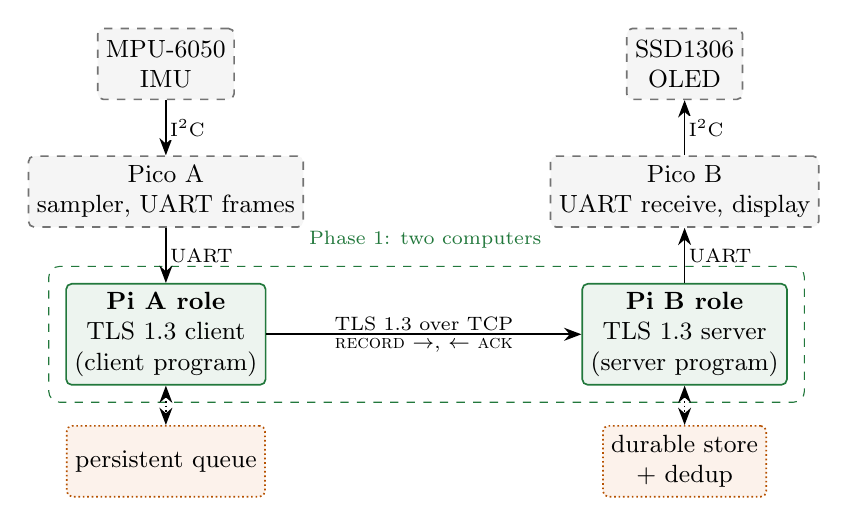
\begin{tikzpicture}[node distance=7mm and 40mm]
  \node[todo] (imu) {MPU-6050\\IMU};
  \node[todo, below=of imu] (pa) {Pico A\\sampler, UART frames};
  \node[done, below=of pa] (pia) {\textbf{Pi A role}\\TLS 1.3 client\\(client program)};
  \node[done, right=of pia] (pib) {\textbf{Pi B role}\\TLS 1.3 server\\(server program)};
  \node[todo, above=of pib] (pb) {Pico B\\UART receive, display};
  \node[todo, above=of pb] (oled) {SSD1306\\OLED};
  \node[next, below=of pia, yshift=2mm] (q) {persistent queue};
  \node[next, below=of pib, yshift=2mm] (st) {durable store\\+ dedup};
  \draw[arr] (imu) -- node[lbl, right] {I\textsuperscript{2}C} (pa);
  \draw[arr] (pa) -- node[lbl, right] {UART} (pia);
  \draw[arr] (pia) -- node[lbl, above] {TLS 1.3 over TCP} node[lbl, below] {\textsc{record} $\rightarrow$, $\leftarrow$ \textsc{ack}} (pib);
  \draw[arr] (pib) -- node[lbl, right] {UART} (pb);
  \draw[arr] (pb) -- node[lbl, right] {I\textsuperscript{2}C} (oled);
  \draw[darr, densely dotted] (pia) -- (q);
  \draw[darr, densely dotted] (pib) -- (st);
  \begin{scope}[on background layer]
    \node[draw=okgreen, dashed, rounded corners=4pt, fit=(pia)(pib), inner sep=6pt,
          ] {};
    \node[font=\scriptsize, okgreen] at ($(pia.north)!0.5!(pib.north)+(0,0.55)$) {Phase 1: two computers};
  \end{scope}
\end{tikzpicture}
\caption{System architecture. Solid green: built and tested in Phase 1. Dotted orange:
next. Dashed grey: Phase 2 hardware.}
\label{fig:system}
\end{figure}

Figure~\ref{fig:modules} shows how the software is layered. The programs never call OpenSSL
directly: one small module, \texttt{tls\_link}, fixes every setting the experiment must keep
constant, so a mistake cannot quietly change what is measured.

\begin{figure}[h]
\centering
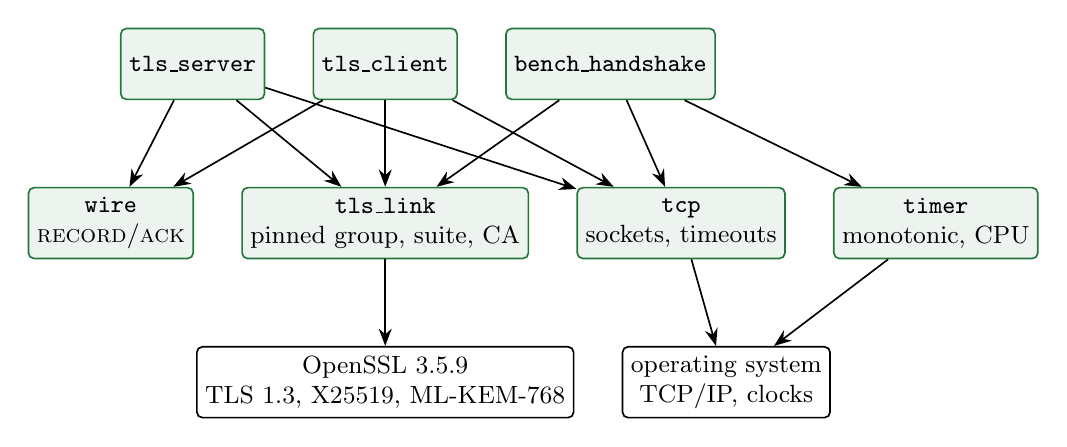
\begin{tikzpicture}[node distance=5mm and 6mm]
  \node[done] (srv) {\texttt{tls\_server}};
  \node[done, right=of srv] (cli) {\texttt{tls\_client}};
  \node[done, right=of cli] (bench) {\texttt{bench\_handshake}};
  \node[done, below=11mm of cli] (tls) {\texttt{tls\_link}\\pinned group, suite, CA};
  \node[done, left=of tls] (wire) {\texttt{wire}\\\textsc{record}/\textsc{ack}};
  \node[done, right=of tls] (tcp) {\texttt{tcp}\\sockets, timeouts};
  \node[done, right=of tcp] (tim) {\texttt{timer}\\monotonic, CPU};
  \node[box, below=11mm of tls] (ossl) {OpenSSL 3.5.9\\TLS 1.3, X25519, ML-KEM-768};
  \node[box, right=of ossl] (os) {operating system\\TCP/IP, clocks};
  \foreach \a/\b in {srv/tls, cli/tls, bench/tls, srv/wire, cli/wire, srv/tcp, cli/tcp,
                     bench/tcp, bench/tim, tls/ossl, tcp/os, tim/os}
    \draw[arr] (\a) -- (\b);
\end{tikzpicture}
\caption{Software layers. Arrows point from a user to what it uses.}
\label{fig:modules}
\end{figure}

\section{Security design}

\subsection{What is fixed}

Configurations A and B differ in exactly one setting, the key-exchange group.
Everything else in Table~\ref{tab:pinned} is identical, as required for a fair comparison.

\begin{table}[h]
\centering
\caption{Settings enforced by \texttt{tls\_link} on both the client and the server.}
\label{tab:pinned}
\small
\begin{tabularx}{\linewidth}{@{}lXX@{}}
\toprule
Setting & Configuration A (classical) & Configuration B (hybrid) \\
\midrule
TLS version & 1.3 only (min = max) & 1.3 only (min = max) \\
Key-exchange group & \texttt{X25519} only & \texttt{X25519MLKEM768} only \\
Cipher suite & \texttt{TLS\_AES\_128\_GCM\_SHA256} & \texttt{TLS\_AES\_128\_GCM\_SHA256} \\
Session tickets, resumption & Off: every handshake is a full one & Off \\
Server certificate & Pinned demo CA, hostname checked & Pinned demo CA, hostname checked \\
Fallback to another group & Never & Never \\
\bottomrule
\end{tabularx}
\end{table}

\subsection{Fail closed, with two independent checks}

Figure~\ref{fig:policy} shows what a client does. A peer that cannot meet the policy ends the
connection; there is no retry with a weaker group and no way to switch verification off. After
the handshake, the negotiated version, group and cipher suite are checked a second time against
the pinned values, and a client confirms that a verified peer certificate exists. Removing one
check by mistake therefore does not open a hole.

\begin{figure}[h]
\centering
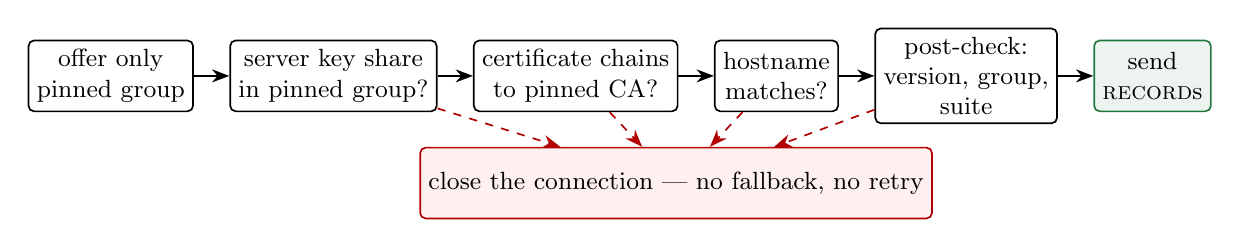
\begin{tikzpicture}[node distance=4mm and 4.5mm, every node/.append style={font=\scriptsize}]
  \node[box] (c1) {offer only\\pinned group};
  \node[box, right=of c1] (c2) {server key share\\in pinned group?};
  \node[box, right=of c2] (c3) {certificate chains\\to pinned CA?};
  \node[box, right=of c3] (c4) {hostname\\matches?};
  \node[box, right=of c4] (c5) {post-check:\\version, group,\\suite};
  \node[done, right=of c5] (ok) {send\\\textsc{record}s};
  \node[box, draw=red!70!black, fill=red!6, below=9mm of $(c3)!0.5!(c4)$] (fail) {close the connection --- no fallback, no retry};
  \foreach \a/\b in {c1/c2, c2/c3, c3/c4, c4/c5, c5/ok} \draw[arr] (\a) -- (\b);
  \foreach \s in {c2, c3, c4, c5} \draw[arr, red!70!black, dashed] (\s) -- (fail);
\end{tikzpicture}
\caption{Client-side checks, in order. Any failure ends the connection.}
\label{fig:policy}
\end{figure}

\subsection{What the handshake carries}

Figure~\ref{fig:handshake} shows the TLS~1.3 handshake. The only visible difference between the
two configurations is the size of the key shares: the hybrid client sends an ML-KEM-768
encapsulation key (1184 bytes, FIPS~203) next to its X25519 key, and the server answers with
an ML-KEM-768 ciphertext (1088 bytes).

\begin{figure}[h]
\centering
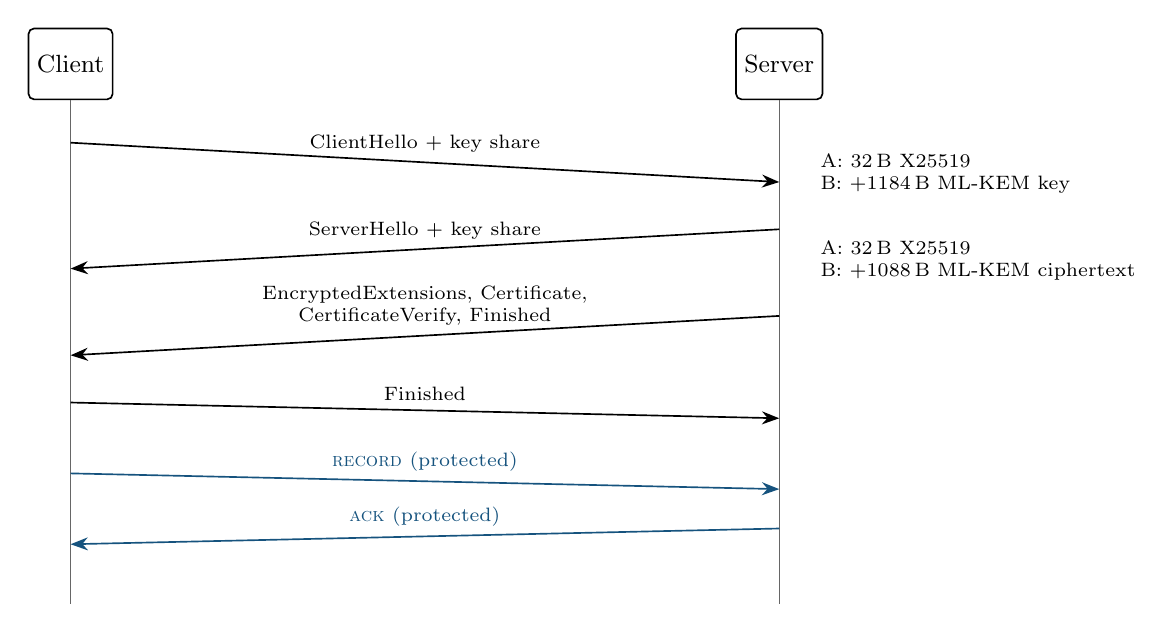
\begin{tikzpicture}[x=1cm,y=1cm]
  \node[box] (C) at (0,0) {Client};
  \node[box] (S) at (9,0) {Server};
  \draw[line width=0.5pt, black!60] (C.south) -- ++(0,-6.4);
  \draw[line width=0.5pt, black!60] (S.south) -- ++(0,-6.4);
  \draw[arr] (0,-1.0) -- node[above, font=\scriptsize] {ClientHello + key share} (9,-1.5);
  \draw[arr] (9,-2.1) -- node[above, font=\scriptsize] {ServerHello + key share} (0,-2.6);
  \draw[arr] (9,-3.2) -- node[above, font=\scriptsize, align=center]
        {EncryptedExtensions, Certificate,\\CertificateVerify, Finished} (0,-3.7);
  \draw[arr] (0,-4.3) -- node[above, font=\scriptsize] {Finished} (9,-4.5);
  \draw[arr, colorA!70!black] (0,-5.2) -- node[above, font=\scriptsize] {\textsc{record} (protected)} (9,-5.4);
  \draw[arr, colorA!70!black] (9,-5.9) -- node[above, font=\scriptsize] {\textsc{ack} (protected)} (0,-6.1);
  \node[font=\scriptsize, align=left, anchor=west] at (9.4,-1.4)
       {A: 32\,B X25519\\B: +1184\,B ML-KEM key};
  \node[font=\scriptsize, align=left, anchor=west] at (9.4,-2.5)
       {A: 32\,B X25519\\B: +1088\,B ML-KEM ciphertext};
\end{tikzpicture}
\caption{TLS~1.3 handshake and the first application messages. Everything after ServerHello
is encrypted.}
\label{fig:handshake}
\end{figure}

\subsection{Message format}

The application protocol is deliberately small. Every message is
\emph{type, length, payload}, big-endian, and a receiver checks the announced length against the
exact size for that type before it reads the payload. A \textsc{record} is 36 bytes on the wire
and an \textsc{ack} is 12 (Figure~\ref{fig:wire}). In Phase 1 the six IMU values are zero, since
no sensor exists yet.

\begin{figure}[h]
\centering
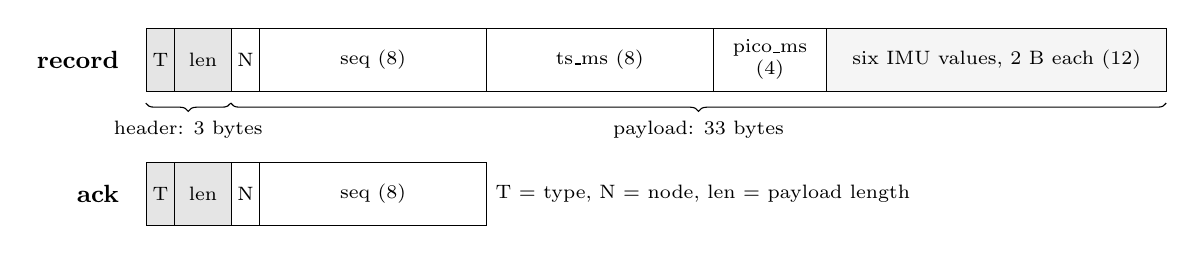
\begin{tikzpicture}[x=0.36cm,y=1cm]
  \tikzset{f/.style={draw, minimum height=8mm, font=\scriptsize, align=center, inner sep=0pt, anchor=west}}
  % one byte = 1 unit = 0.36 cm
  \node[font=\small\bfseries, anchor=east] at (-0.6,0) {\textsc{record}};
  \node[f, minimum width=0.36cm, fill=black!10] at (0,0) {T};
  \node[f, minimum width=0.72cm, fill=black!10] at (1,0) {len};
  \node[f, minimum width=0.36cm] at (3,0) {N};
  \node[f, minimum width=2.88cm] at (4,0) {seq (8)};
  \node[f, minimum width=2.88cm] at (12,0) {ts\_ms (8)};
  \node[f, minimum width=1.44cm] at (20,0) {pico\_ms\\(4)};
  \node[f, minimum width=4.32cm, fill=black!4] at (24,0) {six IMU values, 2 B each (12)};
  \node[font=\small\bfseries, anchor=east] at (-0.6,-1.7) {\textsc{ack}};
  \node[f, minimum width=0.36cm, fill=black!10] at (0,-1.7) {T};
  \node[f, minimum width=0.72cm, fill=black!10] at (1,-1.7) {len};
  \node[f, minimum width=0.36cm] at (3,-1.7) {N};
  \node[f, minimum width=2.88cm] at (4,-1.7) {seq (8)};
  \draw[decorate, decoration={brace, amplitude=3pt, mirror}] (0,-0.55) -- node[below=3pt, font=\scriptsize] {header: 3 bytes} (3,-0.55);
  \draw[decorate, decoration={brace, amplitude=3pt, mirror}] (3,-0.55) -- node[below=3pt, font=\scriptsize] {payload: 33 bytes} (36,-0.55);
  \node[font=\scriptsize, anchor=west] at (12,-1.7) {T = type, N = node, len = payload length};
\end{tikzpicture}
\caption{Wire format. Grey = header. Widths are proportional to bytes. Sequence numbers start at 1;
a \textsc{record} with sequence 0 is rejected.}
\label{fig:wire}
\end{figure}

\section{How it was verified}

Table~\ref{tab:tests} maps each requirement to an automated check. All 10 automated tests (two of them only generate demo certificates) pass on the development
computer. The failure cases run as library tests over a socket pair; the group and certificate
cases also run as real server and client processes over TCP.

\begin{table}[h]
\centering
\caption{Requirements and how they are checked. ``Dev'' = development computer only.}
\label{tab:tests}
\small
\begin{tabularx}{\linewidth}{@{}llXl@{}}
\toprule
Test & Requirement & Automated check & State \\
\midrule
T02 & Log the negotiated group & Group and suite read back after the handshake, both configs & Dev \\
T03 & Wrong hostname or untrusted CA fails closed & Client rejects with a verification error; server sees no session & Dev \\
T04 & Classical-only vs hybrid-only fails & Both directions rejected, no silent downgrade & Dev \\
T09 & Tampered TLS ciphertext rejected & Corrupted record is an I/O error, never delivered & Dev \\
T10 & 100+ handshakes, A vs B & Harness built and exercised; see Section~\ref{sec:results} & Prelim. \\
T05 & Replayed record counted once & Needs the durable store & Next \\
T06--T08 & Outage, restart, 10\%/30\% loss & Needs queue and loss emulation & Planned \\
T01 & Tilt changes the display & Needs Pico, IMU, OLED (Phase 2) & Deferred \\
\bottomrule
\end{tabularx}
\end{table}

\section{Performance measurement}
\label{sec:results}

\subsection{Method}

Figure~\ref{fig:bench} shows one measured attempt. Configurations A and B are \emph{interleaved}
(A, B, A, B, \dots) so that slow changes in load or temperature affect both equally. Every attempt
is a fresh TCP connection and a full handshake. Nothing is written or printed inside the timed
span; rows are kept in memory and saved afterwards. Failed attempts go to a separate file and are
never mixed into the statistics. The first five successes per configuration are warm-up and are
excluded.

\begin{figure}[h]
\centering
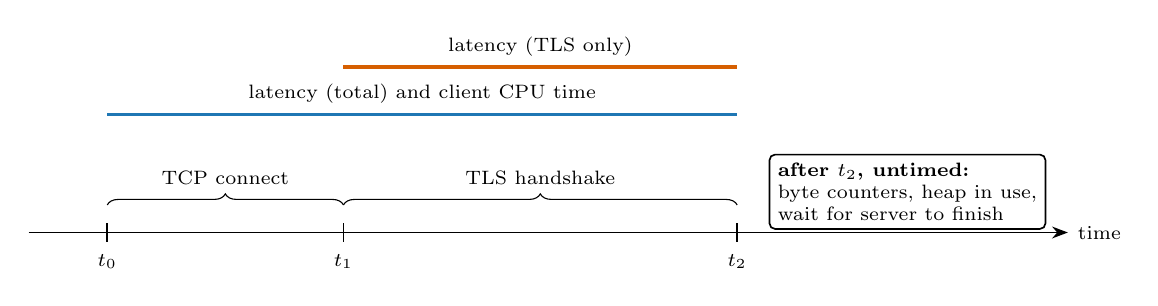
\begin{tikzpicture}[x=1cm,y=1cm]
  \draw[-{Stealth}, line width=0.6pt] (0,0) -- (13.2,0) node[right, font=\scriptsize] {time};
  \foreach \x/\n in {1/t_0, 4/t_1, 9/t_2} {
    \draw[line width=0.6pt] (\x,-0.12) -- (\x,0.12);
    \node[font=\scriptsize, below] at (\x,-0.15) {$\n$};
  }
  \draw[decorate, decoration={brace, amplitude=4pt}] (1,0.35) -- node[above=4pt, font=\scriptsize] {TCP connect} (4,0.35);
  \draw[decorate, decoration={brace, amplitude=4pt}] (4,0.35) -- node[above=4pt, font=\scriptsize] {TLS handshake} (9,0.35);
  \draw[colorA, line width=1.2pt] (1,1.5) -- node[above, font=\scriptsize, black] {latency (total) and client CPU time} (9,1.5);
  \draw[colorB, line width=1.2pt] (4,2.1) -- node[above, font=\scriptsize, black] {latency (TLS only)} (9,2.1);
  \node[box, align=left, font=\scriptsize, anchor=north west] at (9.4,1.0)
      {\textbf{after $t_2$, untimed:}\\ byte counters, heap in use,\\ wait for server to finish};
\end{tikzpicture}
\caption{One measured handshake attempt.}
\label{fig:bench}
\end{figure}

Per attempt the client records: total latency ($t_0$ to $t_2$) and TLS-only latency ($t_1$ to
$t_2$); client CPU time over the same span; handshake bytes sent and received, counted by OpenSSL
on the socket (the TLS byte stream, without TCP/IP headers); and the heap held by the open
connection. The transient memory peak inside the handshake is not captured per attempt. Server-side
CPU and memory are not measured yet.

\subsection{Conditions}

\begin{itemize}\setlength\itemsep{0pt}
\item Platform: \CpuModel, WSL2; client and both servers on one machine over loopback.
\item OpenSSL 3.5.9; Release build; git commits \GitCommits{} (working tree modified: \GitDirty).
\item \NSessions{} separate sessions of \NPerSession{} measured handshakes per configuration
      (\NPerConfig{} per configuration in total), no failures. Measured on \RunDate.
\item Negotiated groups seen: \texttt{\GroupA} (A) and \texttt{\GroupB} (B).
\end{itemize}

\textbf{Preliminary:} one development computer, loopback network, no packet loss. These
numbers show that the harness works and what the size and cost of the hybrid handshake look like
here. They are not results for the target hardware and must not be quoted as such.

\subsection{Handshake size}

The byte counts are deterministic, so they are the most solid result so far. Figure~\ref{fig:bytes}
shows that the hybrid handshake sends \DeltaTx{} bytes more and receives \DeltaRx{} bytes more than
the classical one. These differences are exactly the ML-KEM-768 encapsulation key and ciphertext
that the handshake carries.

\begin{figure}[h]
\centering
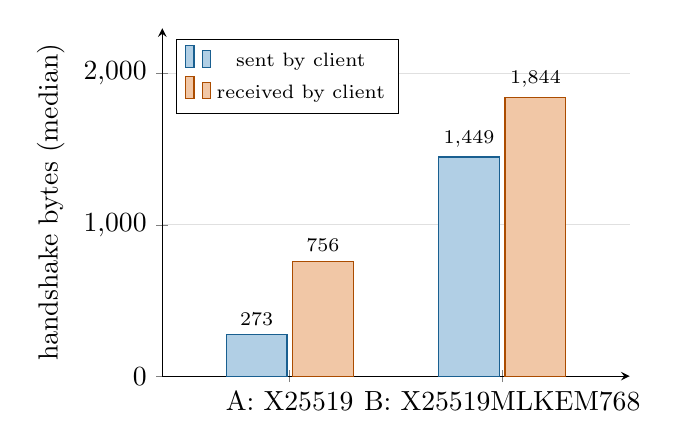
\begin{tikzpicture}
  \begin{axis}[ybar, width=0.62\linewidth, height=6cm, bar width=22pt,
      xtick={1,2}, xticklabels={A: X25519, B: X25519MLKEM768}, xmin=0.4, xmax=2.6,
      ylabel={handshake bytes (median)}, ymin=0, ymax=2300,
      legend style={at={(0.03,0.97)}, anchor=north west, font=\scriptsize},
      nodes near coords, every node near coord/.append style={font=\scriptsize},
      axis lines=left, ymajorgrids, grid style={black!12}]
    \addplot[fill=colorA!35, draw=colorA!80!black] coordinates {(1,\BytesTxA) (2,\BytesTxB)};
    \addplot[fill=colorB!35, draw=colorB!80!black] coordinates {(1,\BytesRxA) (2,\BytesRxB)};
    \legend{sent by client, received by client}
  \end{axis}
\end{tikzpicture}
\caption{Handshake bytes on the TLS stream, median over \NPerConfig{} handshakes per configuration.}
\label{fig:bytes}
\end{figure}

\subsection{Latency and CPU time}

Figure~\ref{fig:box} shows the spread of the \NPerConfig{} handshakes per configuration. The
hybrid handshake is slower, with a median total latency of \MedTotB{}\,ms against \MedTotA{}\,ms
(95th percentiles \PNineFiveTotB{} and \PNineFiveTotA{}\,ms). Client CPU time is \MedCpuB{}\,ms
against \MedCpuA{}\,ms. The open connection holds about \MedHeapB{}\,KiB of heap in configuration~B
and \MedHeapA{}\,KiB in configuration~A.

\begin{figure}[h]
\centering
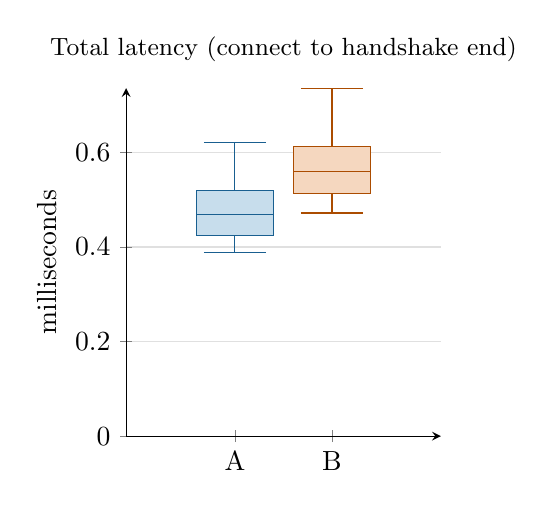
\begin{tikzpicture}
  \begin{axis}[boxplot/draw direction=y, width=0.46\linewidth, height=6cm,
      xtick={1,2}, xticklabels={A, B}, ymin=0, ylabel={milliseconds},
      title={\small Total latency (connect to handshake end)},
      axis lines=left, ymajorgrids, grid style={black!12}, enlarge x limits=0.4]
    % Generated by prepare_data.py. Do not edit.
\addplot+[boxplot prepared={draw position=1, lower whisker=0.3879, lower quartile=0.4238, median=0.4690, upper quartile=0.5198, upper whisker=0.6202}, fill=colorA!25, draw=colorA!80!black] coordinates {};
\addplot+[boxplot prepared={draw position=2, lower whisker=0.4718, lower quartile=0.5128, median=0.5590, upper quartile=0.6122, upper whisker=0.7359}, fill=colorB!25, draw=colorB!80!black] coordinates {};

  \end{axis}
\end{tikzpicture}\hfill
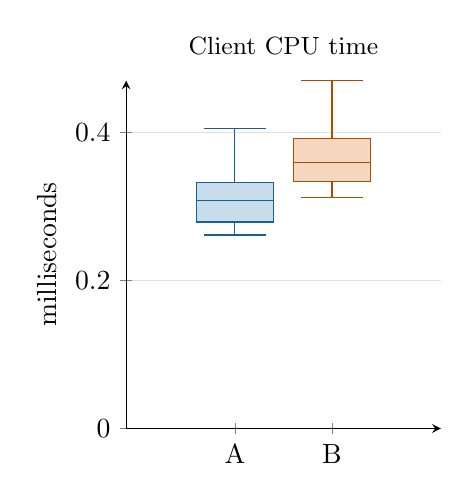
\begin{tikzpicture}
  \begin{axis}[boxplot/draw direction=y, width=0.46\linewidth, height=6cm,
      xtick={1,2}, xticklabels={A, B}, ymin=0, ylabel={milliseconds},
      title={\small Client CPU time},
      axis lines=left, ymajorgrids, grid style={black!12}, enlarge x limits=0.4]
    % Generated by prepare_data.py. Do not edit.
\addplot+[boxplot prepared={draw position=1, lower whisker=0.2615, lower quartile=0.2790, median=0.3076, upper quartile=0.3326, upper whisker=0.4057}, fill=colorA!25, draw=colorA!80!black] coordinates {};
\addplot+[boxplot prepared={draw position=2, lower whisker=0.3123, lower quartile=0.3336, median=0.3588, upper quartile=0.3913, upper whisker=0.4701}, fill=colorB!25, draw=colorB!80!black] coordinates {};

  \end{axis}
\end{tikzpicture}
\caption{Distribution over all \NPerConfig{} handshakes per configuration. Box: 25th to 75th
percentile with the median line; whiskers: 5th and 95th percentile. A = classical,
B = hybrid. Preliminary, development computer.}
\label{fig:box}
\end{figure}

\subsection{Repeatability}

A single session can mislead, so Figure~\ref{fig:sessions} shows each of the \NSessions{}
sessions separately. The absolute values move from session to session, but configuration~B is
slower than A in every session. The B-to-A ratio of the median latency stays between
\RatioMin{} and \RatioMax{} (median \RatioMedian{}). That is a consistent trend, but on one
machine with a loopback network it says little about how a Raspberry Pi over Wi-Fi will behave.

\begin{figure}[h]
\centering
\begin{tikzpicture}
  \begin{axis}[width=0.8\linewidth, height=6.2cm, xlabel={session}, ylabel={total latency (ms)},
      xtick={1,2,3,4,5}, ymin=0, ymax=1.0, axis lines=left, ymajorgrids, grid style={black!12},
      legend style={at={(0.03,0.97)}, anchor=north west, font=\scriptsize, draw=black!30},
      legend columns=2, mark size=2pt]
    \addplot[colorA, mark=*] table[col sep=comma, x=session, y=med_total_ms]{data/sessions_A.csv};
    \addplot[colorA, mark=triangle*, dashed] table[col sep=comma, x=session, y=p95_total_ms]{data/sessions_A.csv};
    \addplot[colorB, mark=*] table[col sep=comma, x=session, y=med_total_ms]{data/sessions_B.csv};
    \addplot[colorB, mark=triangle*, dashed] table[col sep=comma, x=session, y=p95_total_ms]{data/sessions_B.csv};
    \legend{A median, A p95, B median, B p95}
  \end{axis}
\end{tikzpicture}
\caption{Median and 95th-percentile total latency in each session (\NPerSession{} handshakes per
configuration per session).}
\label{fig:sessions}
\end{figure}

\section{Claims and limits}

\begin{itemize}\setlength\itemsep{0pt}
\item \textbf{Hybrid key establishment is not post-quantum authentication.} The server
      certificate is a classical ECDSA P-256 demo certificate. Only the key exchange is hybrid.
\item This is an educational link. It is not flight-approved, not space-qualified and not
      endorsed by any agency.
\item Results come from a development computer over loopback. Nothing here is gate evidence;
      that requires the target hardware, recorded board identifiers and the instructor's initials.
\item The server's acknowledgment is not yet tied to durable storage, so it does not yet mean
      ``committed''.
\item Handshake bytes exclude TCP/IP headers; a packet capture is still needed for those totals.
\item Server-side CPU and memory are not measured yet.
\end{itemize}

\section{Roadmap}

Figure~\ref{fig:roadmap} places the work against the ten build gates. A software part being
implemented does not mean the gate is passed: each gate still needs its hardware evidence.

\begin{figure}[h]
\centering
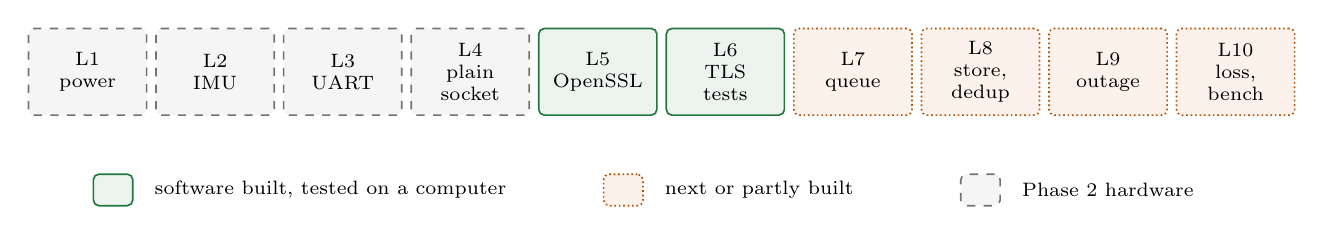
\begin{tikzpicture}[x=1.62cm, y=1cm]
  \tikzset{g/.style={minimum width=1.5cm, minimum height=1.1cm}}
  \foreach \n/\s/\t in {1/todo/{L1\\power}, 2/todo/{L2\\IMU}, 3/todo/{L3\\UART}, 4/todo/{L4\\plain\\socket},
                       5/done/{L5\\OpenSSL}, 6/done/{L6\\TLS\\tests}, 7/next/{L7\\queue}, 8/next/{L8\\store,\\dedup},
                       9/next/{L9\\outage}, 10/next/{L10\\loss,\\bench}} {
    \node[\s, g, font=\scriptsize] at (\n,0) {\t};
  }
  \node[done, minimum width=0.5cm, minimum height=0.4cm] at (1.2,-1.5) {};
  \node[font=\scriptsize, anchor=west] at (1.45,-1.5) {software built, tested on a computer};
  \node[next, minimum width=0.5cm, minimum height=0.4cm] at (5.2,-1.5) {};
  \node[font=\scriptsize, anchor=west] at (5.45,-1.5) {next or partly built};
  \node[todo, minimum width=0.5cm, minimum height=0.4cm] at (8.0,-1.5) {};
  \node[font=\scriptsize, anchor=west] at (8.25,-1.5) {Phase 2 hardware};
\end{tikzpicture}
\caption{Build gates L1--L10. Gate L10 (benchmark) is partly built: the handshake harness exists,
the loss runs do not.}
\label{fig:roadmap}
\end{figure}

\textbf{Next steps.}
\begin{enumerate}\setlength\itemsep{0pt}
\item Durable store with duplicate detection, so an acknowledgment means the record is stored (T05).
\item Persistent queue, outage recovery and packet-loss tests (T06--T08).
\item Repeated benchmark runs with server-side CPU and memory, and packet captures for byte totals.
\item Review with the advisor, then plan the Pico~W migration.
\end{enumerate}

\textbf{Questions for the advisor.} How should packet loss be emulated (\texttt{tc netem} on the
computers or at the access point)? May the Pi services stay in C? May we reuse the existing CSV
logger for evidence files? Is a second computer needed for the final Phase~1 measurements?

\end{document}
